\documentclass[10pt]{article}
\usepackage[margin=0.8in]{geometry}
\usepackage{graphicx}
\usepackage{hyperref}
\usepackage{longtable}
\title{Four archived prior-art metadata corrections}
\author{Source-bound validation note}
\date{2026-10-23}
\begin{document}
\maketitle
\noindent\textbf{Scope.} Four frozen October 6 proposals had a descriptive frontier-map value and untyped nearest-prior-work relations. The originals remain unchanged. Hash-bound replacements name the actual index-calculus directory, use KB provenance and the adjacent relation, and preserve each original description in a detail field. No trial, proof, numerical claim, or hypothesis status changes.\par
\medskip
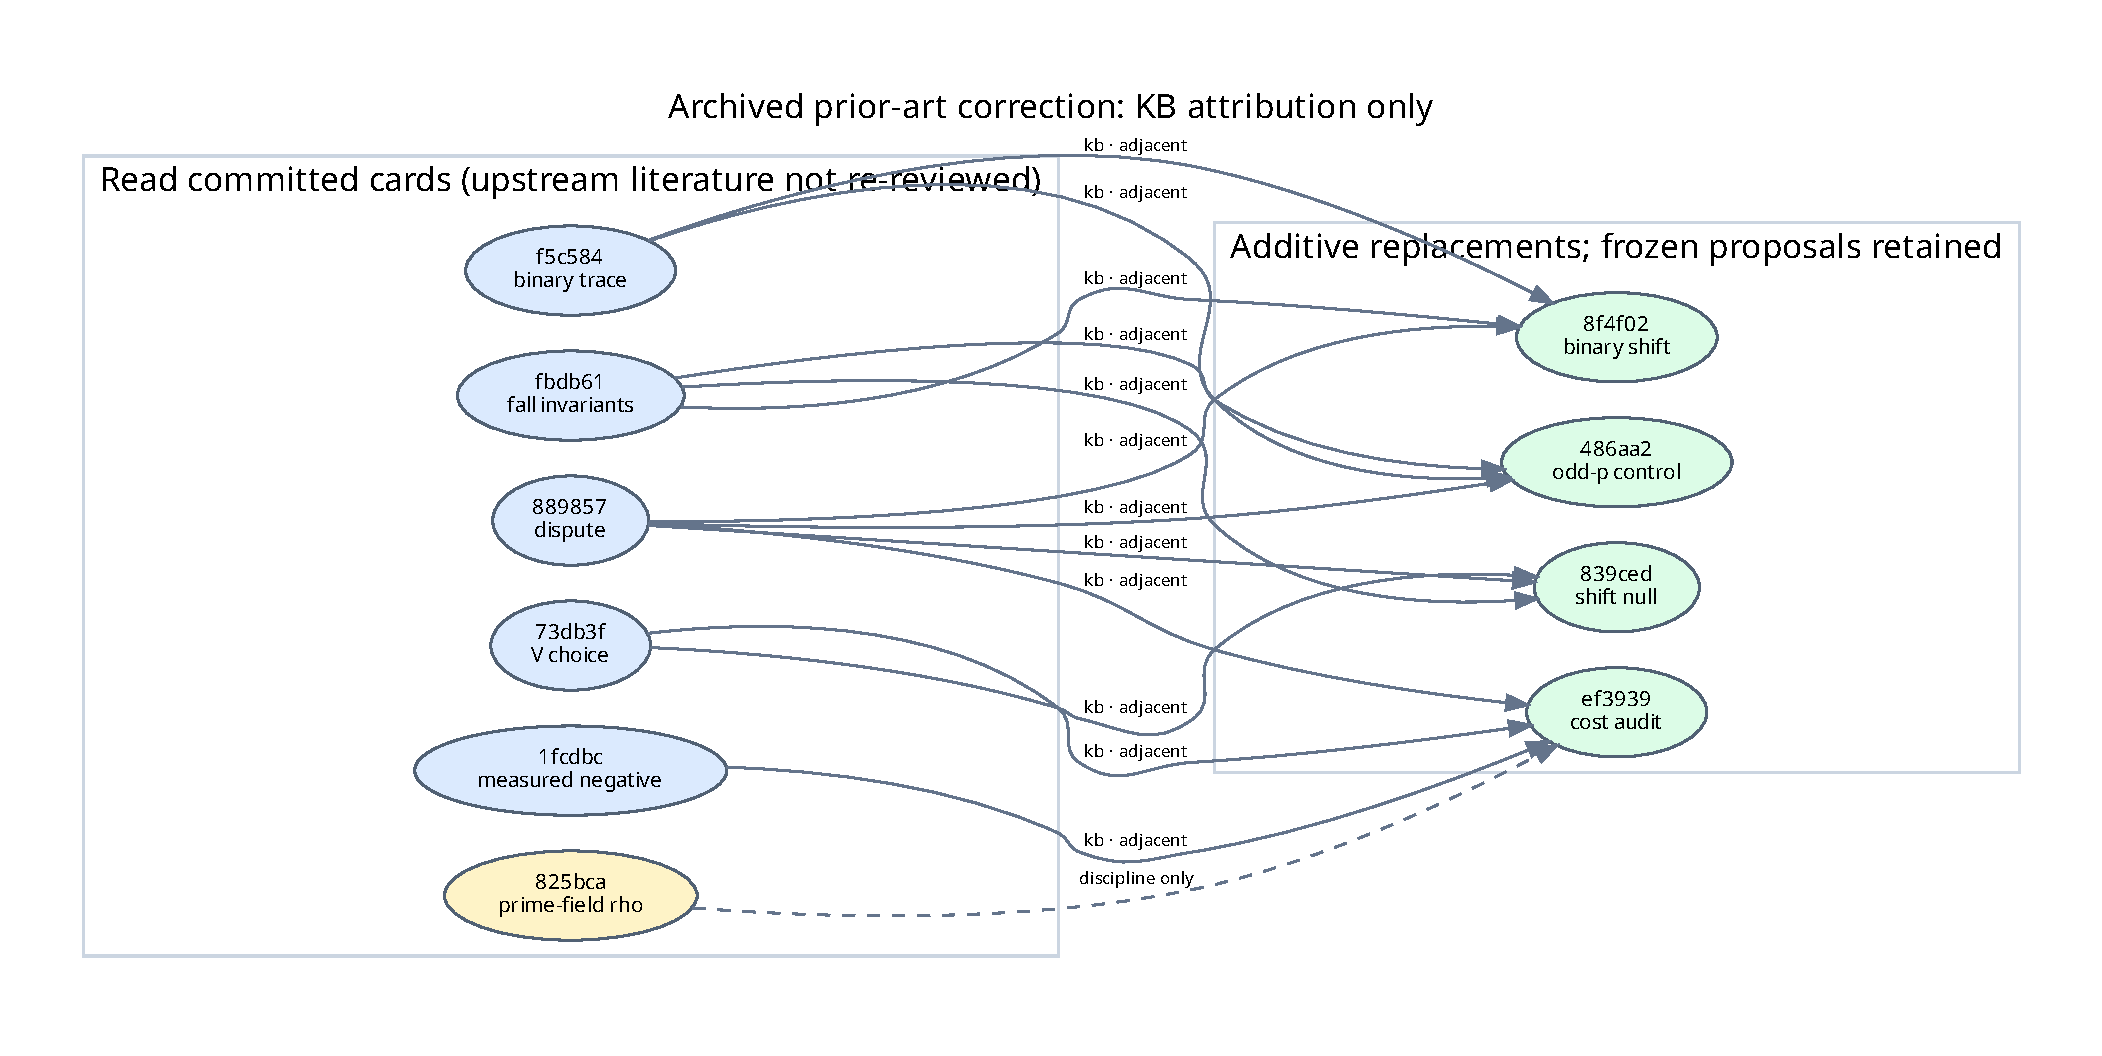
\includegraphics[width=\textwidth]{prior-art-graph.pdf}
\medskip
\noindent\textbf{Source boundary.} Six committed knowledge cards were read. Their upstream literature has mixed reading states and was not independently re-reviewed. The prime-field rho card contributes accounting discipline only; its constants are not transferred to a binary baseline.\par
\medskip
\noindent\textbf{Validation.} On parent commit \texttt{9fc0685a5fd5}, the complete-tree ledger gate reported 118 unsuppressed errors. With these replacements it reported 88: exactly 30 targeted lines removed and zero added. Both runs exited 1. A focused checker confirms SHA-256 bindings and all non-prior-art parsed fields. The broader ledger and theorem-to-claim fidelity remain open.\par
\medskip
\noindent\textbf{Evidence.} See \texttt{REPORT.md}, \texttt{validation.json}, the two validator logs, the six named KR cards, and the four registered supersessions in this PR.\par
\end{document}
